
\documentclass{article}
\usepackage{amsmath, amssymb,amsfonts,mdframed, tikz}
\usepackage[ruled,linesnumbered]{algorithm2e}
\usetikzlibrary{shapes,arrows,calc,positioning,backgrounds}
\title{Algorithms \& Complexity: Lecture 7, Greedy Algorithms I}

\author{Sam Barrett}

\newcommand{\T}{\texttt{T }}
\newcommand{\True}{\texttt{True }}
\newcommand{\F}{\texttt{F }}
\newcommand{\False}{\texttt{False }}
\newcommand{\NP}{\mathbf{NP}}
\renewcommand{\P}{\mathbf{P}}
\newcommand{\N}{\mathbb{N}}

\newmdtheoremenv{lemma}{Lemma}
\newmdtheoremenv{definition}{Definition}
\newmdtheoremenv{theorem}{Theorem}
\newmdtheoremenv{problem}{Problem}
\newmdtheoremenv{example}{Example}

\begin{document}
\maketitle

\section{What are greedy algorithms?}

There is no formal definition for greedy algorithms, we can actually design multiple different greedy algorithms to solve the same problem. They are categorised as algorithms that make local decisions to improve a solution, working step-by-step with no concern for what they have done previously or might do later. Often this short-sighted approach does not help in finding an optimal solution, however, some can still approximate an optimal solution.

There are advantages and disadvantages of greedy algorithms.

Advantages:

\begin{itemize}
  \item They are intuitive
  \item This leads to them being easy to explain and implement
  \item Most heuristics are based on \textit{greedy} choices
  \item They can be shown to sometimes be approximately correct
\end{itemize}

Disadvantages:

\begin{itemize}
  \item There are different notions of greedy, no formal definition
  \item Local correct steps do not guarantee a globally correct approach
  \item Often do not result in optimal solutions
\end{itemize}

Our 2-approximation for the vertex cover problem discussed in the previous lecture is an example of a greedy algorithm, it ran in polynomial time.

\section{Dijkstra's Algorithm}

This is an algorithm that finds the shortest paths in a directed graph from a fixed vertex $s$.

\begin{algorithm}
  \caption{Dijkstra's Algorithm}
  Let $S$ be the set of explored vertices

  For each $u \in S$ we store the distance of the shortest $s \rightarrow u$ path in $\texttt{dist}(u)$

  Initialise $S= \{ s \} $ and $\texttt{dist}(s) = 0 $

  \While{$S\neq V$}{
    Select a vertex $v \notin S$ which minimises $\texttt{temp-dist}(v) = \displaystyle\min_{(u,v) \in E, u \in S}(\texttt{dist}(u) + \texttt{length}(u,v)  )$

    Add $v$ to $S$ and set $\texttt{dist}(v) = \texttt{temp-dist}(v)  $
  }
\end{algorithm}


The running time of this algorithm is $O(mn)$ where $n,m$ are the number of vertices and edges respectively. This is the case as the while loop runs at most $n$ times and each iteration takes $m$ steps.

\subsection{Correctness of Dijkstra's algorithm}

\begin{theorem}
Consider the set $S$ at any point in the running of the algorithm. For each $u \in S$ the quantity $\texttt{dist} (u)$ stores the value of the shortest $s \rightarrow u$ path.
\end{theorem}

We can prove this by induction:

\begin{itemize}
  \item \underline{Base case:} $|S| =1$ and $\texttt{dist}(s) =0 $

  \item \underline{Inductive hypothesis:} Suppose that the theorem holds for $|S| = k$
  \item \underline{Inductive step:} Suppose we now grow $S$ by one more vertex by adding some vertex $v$.

        By line 5 we know: $\texttt{temp-dist}(v) = \texttt{dist}(u) + \texttt{length}(u,v)   $ for some $u$ already in $S$

        Suppose that there is a path $P$ $s \rightarrow v$ that is shorter than $\texttt{dist}(v) $

        Let $P$ leave $S$ via an edge $(x,y)$ for some $x\in S, y \notin S$

        \textbf{Contradiction}
\end{itemize}

\section{Prim's algorithm}

Prim's algorithm is an algorithm for finding the minimum spanning tree of a given graph $G$.


\subsection{Minimum spanning trees}

Let $G$ be a undirected, connected graph $G = (V,E)$ with $n$ vertices.

A subgraph $T = (V',E')$ of $G$ is said to be a \textbf{spanning tree} if:

\begin{itemize}
  \item spanning $\rightarrow V' = V $
  \item tree $\rightarrow |E'| = n-1$
\end{itemize}

For instance, the graph:

\begin{center}
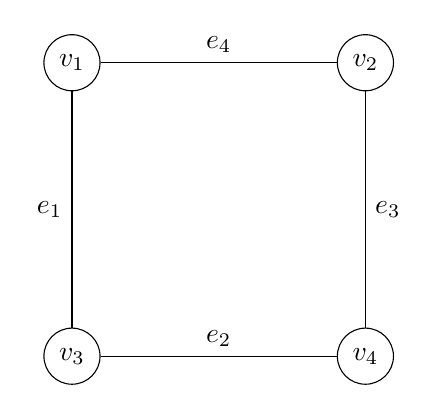
\begin{tikzpicture}
  \node[circle,draw] (v1) {$v_{1}$};
  \node[circle,draw, right = 3cm of v1] (v2) {$v_{2}$};
  \node[circle,draw, below = 3cm of v1] (v3) {$v_{3}$};
  \node[circle,draw, below = 3cm of v2] (v4) {$v_{4}$};

  \draw (v1) -- (v3) node [midway,left] {$e_{1}$};
  \draw (v1) -- (v2) node [midway,above] {$e_{4}$};
  \draw (v2) -- (v4) node [midway,right] {$e_{3}$};
  \draw (v3) -- (v4) node [midway,above] {$e_{2}$};

\end{tikzpicture}
\end{center}

Has 4 different spanning trees:

\begin{enumerate}
  \item
        \begin{center}
        \begin{tikzpicture}
        \node[circle,draw] (v1) {$v_{1}$};
        \node[circle,draw, right = 3cm of v1] (v2) {$v_{2}$};
        \node[circle,draw, below = 3cm of v1] (v3) {$v_{3}$};
        \node[circle,draw, below = 3cm of v2] (v4) {$v_{4}$};

        \draw (v1) -- (v2) node [midway,above] {$e_{4}$};
        \draw (v2) -- (v4) node [midway,right] {$e_{3}$};
        \draw (v3) -- (v4) node [midway,above] {$e_{2}$};

        \end{tikzpicture}
      \end{center}
  \item

\begin{center}
\begin{tikzpicture}
  \node[circle,draw] (v1) {$v_{1}$};
  \node[circle,draw, right = 3cm of v1] (v2) {$v_{2}$};
  \node[circle,draw, below = 3cm of v1] (v3) {$v_{3}$};
  \node[circle,draw, below = 3cm of v2] (v4) {$v_{4}$};

  \draw (v1) -- (v3) node [midway,left] {$e_{1}$};
  \draw (v1) -- (v2) node [midway,above] {$e_{4}$};
  \draw (v2) -- (v4) node [midway,right] {$e_{3}$};

\end{tikzpicture}
\end{center}
  \item
        \begin{center}
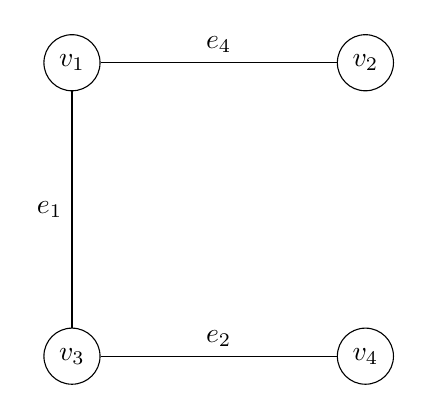
\begin{tikzpicture}
  \node[circle,draw] (v1) {$v_{1}$};
  \node[circle,draw, right = 3cm of v1] (v2) {$v_{2}$};
  \node[circle,draw, below = 3cm of v1] (v3) {$v_{3}$};
  \node[circle,draw, below = 3cm of v2] (v4) {$v_{4}$};

  \draw (v1) -- (v3) node [midway,left] {$e_{1}$};
  \draw (v1) -- (v2) node [midway,above] {$e_{4}$};
  \draw (v3) -- (v4) node [midway,above] {$e_{2}$};

\end{tikzpicture}
\end{center}
  \item
        \begin{center}
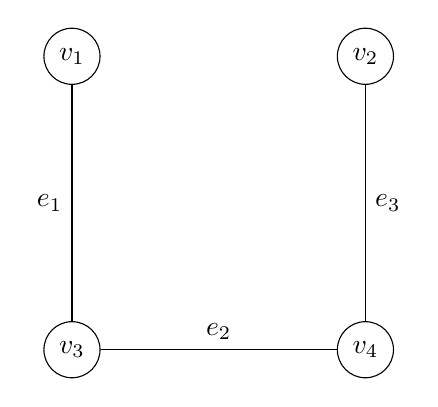
\begin{tikzpicture}
  \node[circle,draw] (v1) {$v_{1}$};
  \node[circle,draw, right = 3cm of v1] (v2) {$v_{2}$};
  \node[circle,draw, below = 3cm of v1] (v3) {$v_{3}$};
  \node[circle,draw, below = 3cm of v2] (v4) {$v_{4}$};

  \draw (v1) -- (v3) node [midway,left] {$e_{1}$};
  \draw (v2) -- (v4) node [midway,right] {$e_{3}$};
  \draw (v3) -- (v4) node [midway,above] {$e_{2}$};

\end{tikzpicture}
\end{center}

\end{enumerate}


\begin{problem}(Minimum Spanning Tree (MST) problem)

Given an undirected, connected graph $G = (V,E)$ with edge costs given by $\texttt{cost}: E \rightarrow \mathbb{R}^{+} $, find a spanning tree $T = (V,E')$ such that $\sum_{e\in E'}\texttt{cost}(e)$ is minimised
\end{problem}

\begin{algorithm}
  \caption{Finding MST - Prim's algorithm}

  Let $S$ be the set of explored vertices

  Initialise $S = \{ s \} $ where $s$ is any vertex

  Initialise $E' = \emptyset$

  \While{$S \neq V$}{
    Select a vertex $v \notin S$ which minimises $\displaystyle\min_{e =u -v, u \in S} \texttt{cost} (e)$

    Add $v$ to $S$ and $e$ to $E'$
  }

\end{algorithm}

Running time of this algorithm is $O(mn)$ where $n,m$ are the number of vertices and edges respectively.
The while loop runs at most $n$ times with each loop requiring $m$ time.

\subsection{Correctness of Prim's algorithm}

We first make an assumption that all edge costs are \textbf{distinct}.

\begin{theorem}
  For any $S \subset V$, let $e$ be the edge of minimum cost having one end point in $S$ and one end point in $V \backslash S$. Then every MST contains the edge $e$
\end{theorem}

First suppose that there is a MST $T$ which does not contain this edge $e$ whose endpoints are $v\in S$ and $w \notin S$. We will now find an edge $e'$ in $T$ s.t. $\texttt{cost} (e') >\texttt{cost} (e)$. Therefore, replacing $e'$ with $e$ gives a spanning tree of lower cost, thus deriving a contradiction.

\section{Kruskal's algorithm}

\begin{algorithm}
  \caption{Kruskal's algorithm}
  Order the edges of $E$ as $e_{1},e_{2},\ldots,e_{m}$ in order of cost (increasing)

  Initialise $E' = \emptyset$ and $i=1$

  \While{$i \leq m$}{
    \uIf{adding $e_{i}$ to $E'$ does not create a cycle }{
      Add $e_{i}$ to $E'$
    }\Else{
      Do not add $e_{i}$ to $E'$
    }
    $i++$
  }
\end{algorithm}

This algorithms also runs in $O(mn)$ time where $n,m$ are the number of vertices and edges respectively.

The notable difference with this algorithm is that we do \textbf{not} consider all edges

\subsection{Correctness of Kruskal's algorithm}

We again make the assumption that all edge-costs are distinct.

\begin{theorem}(Same as for Prim's)
  For any $S \subset V$, let $e$ be the edge of minimum cost having one end point in $S$ and one end point in $V \backslash S$. Then every MST contains the edge $e$
\end{theorem}

We consider the algorithm at some arbitrary step.

Suppose Kruskal's algorithm adds the edge $v - w$ at this step.

Let $S$ be the set of all vertices to which $v$ had a path to before this step. We can see that $w \notin S$ as otherwise we would have a cycle, breaking the algorithm at line 4.

By the definition of $S$ no edges from $S$ to $V \backslash S$ have been added before this stage.

Since $v \in S$ and $w \notin S$ and as Kruskal's algorithm adds edges in increasing order of cost, it follows that $v - w$ is the \textit{cheapest} edge with one endpoint in $S$ and the other in $V \backslash S$

\section{Reverse-delete algorithm for finding MSTs}

We can also approach this problem from the opposite direction. Instead of adding edges until we cannot avoid creating a cycle, we start and remove (the most expensive) edges until no cycles are left.

\end{document}
